\chapter{Implementacija i korisničko sučelje}
		
		
		\section{Korištene tehnologije i alati}
		
		    \texttt{}{
               Komunikacija u timu postignuta je izradom Discord servera NULL grupe 2022./2023. i WhatsApp grupe kojima su pristup imali svi članovi tima. Ova dva kanala komunikacije omogućavali su nam brzu i jednostavnu komunikaciju, te spremnost svakog člana na pomoć drugome u nevolji u kratkom vremenu. Za izradu UML dijagrama koristili smo Draw.io, Astah Professional, Visual Paradigm, Microsoft Paint... Sustav za upravljanje, upravljan je izvornim kodom Git. Repozitorij projekta dostupan je na web platformi GitLab. 

               Razvojno okruženje korišteno pri izradi je Visual Studio Code, integrirano razvojno okruženje tvrtke Microsoft. Prvenstveno se koristi za razvoj računalnih programa za operacijski sustav Windows, kao i za web-stranice, web-aplikacije, web-usluge i mobilne aplikacije. Visual Studio za razvoj softvera koristi Microsoft-ove platforme kao sto su Windows API, Windows Forms, Windows Presentation Foundation, Windows Store i Microsoft Silverlight. Backend domena izrađena je pomoću radnog okvira Node.js i jezika Javascript, a frontend domena korištenjem Angular okvira, te jezikom Typescript. 

              

              
            }

            
             \textit{Linkovi na alate:}
            \newline
             \url{https://code.visualstudio.com/}
             \newline
             \url{https://www.whatsapp.com/}
             \newline
             \url{https://online.visual-paradigm.com/}
             \newline
             \url{https://discord.com/}
             \newline
             \url{https://app.diagrams.net/}
             \newline
             \url{https://astah.net/products/astah-professional/}
             \newline
             \url{https://nodejs.org/en/}
             \newline
             \url{https://angular.io/}
             \newline
             \url{https://gitlab.com/}
             \newline
             \url{https://git-scm.com/}
             
			
			
			\eject 
		

		\section{Ispitivanje programskog rješenja}
	
			
			\subsection{Ispitivanje komponenti}
			Ispitivanje komponenti ostvareno je korištenjem Jest alata za ispitivanje. U nastavku su opisani provedeni testovi te priložene funkcija za tesriranje te izlaz koji se dobije testiranjem. Prikazani testovi pokrivaju klase UserModel i AppointmentModel koje implementiraju najvažnije funkcionalnosti aplikacije
    
            \begin{figure}[H]
                    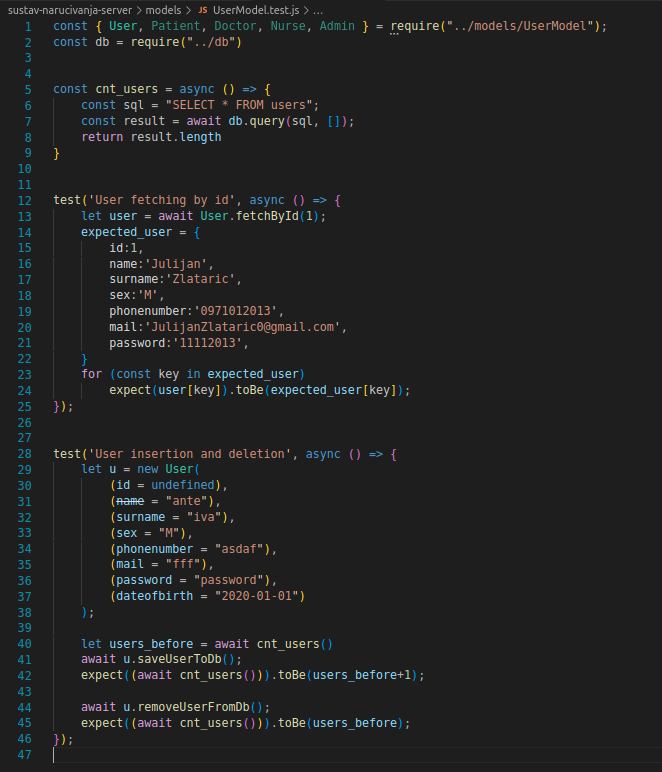
\includegraphics[width=300pt]{slike/usermodel_tests_code.png} %veličina u odnosu na širinu linije
                    \caption{Testovi za klasu korisnika}
                    \label{fig:test1} %label mora biti drugaciji za svaku sliku
                \end{figure}
                Prikazani testovi testiraju dohvačanje usera iz baze podataka te njegovo ubacivanje i izbacivanje iz baze podataka. Navedene funkcionalnosti su nužne za pravilnu registraciju i login korisnika aplikacije.
                \eject

                \begin{figure}[H]
                    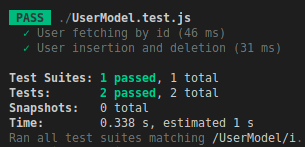
\includegraphics[width=\textwidth]{slike/usermodel_tests_out.png} %veličina u odnosu na širinu linije
                    \caption{Izlaz programa za testiranje klase korisnika}
                    \label{fig:test2} %label mora biti drugaciji za svaku sliku
                \end{figure}
                Izlaz programa za testiranje klase UserModel s 2 testna primjera. Sa slike je vidljivo da klasa prolazi testne primjere.

            \begin{figure}[H]
                    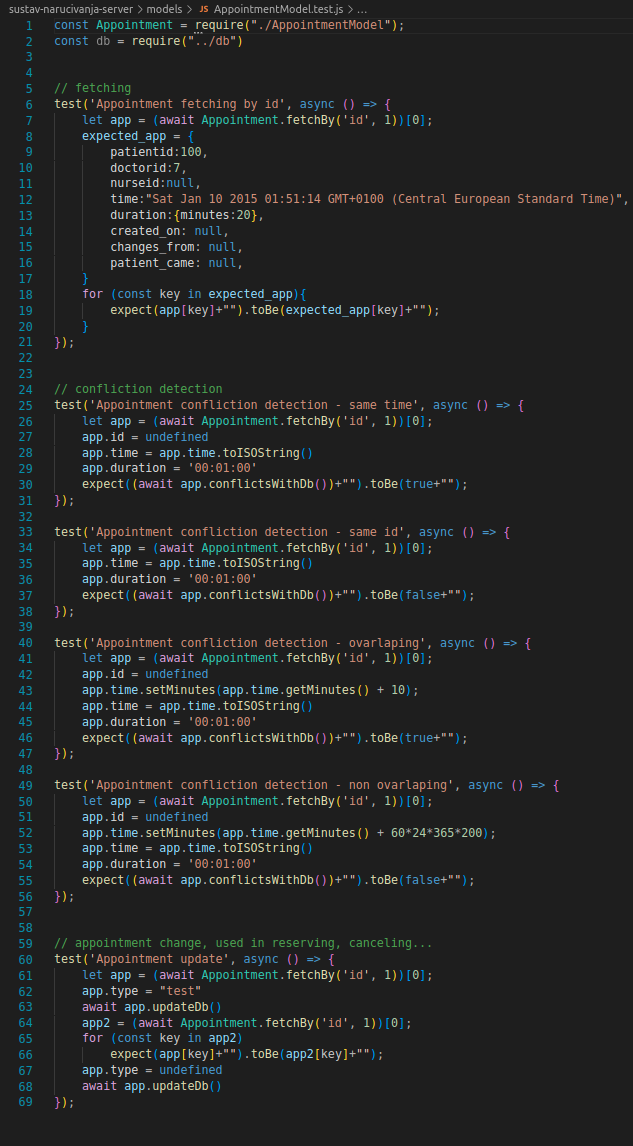
\includegraphics[width=300pt]{slike/appointment_tests_code.png} %veličina u odnosu na širinu linije
                    \caption{Testovi za klasu termina}
                    \label{fig:test3} %label mora biti drugaciji za svaku sliku
                \end{figure}
                Prikazani testovi testiraju dohvačanje određenog termina iz baze podataka, testiranje postoji li određeni termin koji je u vremenskom konfliktu s odabranim terminom te testiranje updateanja termina. Testiranje konflikata ima vise rubnih slučajeva, naime isti termin mogli smo već dohvatiti iz baze podataka te tada nebi trebalo biti konflikata, zatim moguće je da se termin nalazi unutar drugoga, potpuno izvan...

                \begin{figure}[H]
                    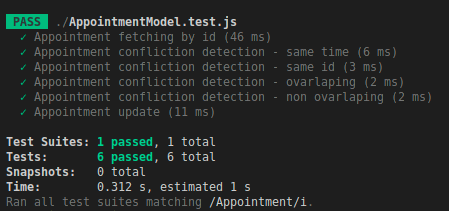
\includegraphics[width=\textwidth]{slike/appointment_tests_out.png} %veličina u odnosu na širinu linije
                    \caption{Izlaz programa za testiranje klase termina}
                    \label{fig:test4} %label mora biti drugaciji za svaku sliku
                \end{figure}
                Izlaz programa za testiranje klase AppointmentModel s 6 testnih primjera. Sa slike je vidljivo da klasa prolazi testne primjere.
			
			
			\subsection{Ispitivanje sustava}
			
			 Ispitivanje sustava provedeno je koristeći radni okvir Selenium\footnote{\url{https://www.seleniumhq.org/}} u obliku dodataka za preglednik \textbf{Selenium IDE} - preko kojeg se izvodilo snimanje korisnikovih akcija radi automatskog ponavljanja ispita. Razrađeno je \textbf{7 ispitnih slučajeva} u kojima su redovni slučajevi, rubni uvjeti te poziv funkcionalnosti koja nije implementirana/izaziva pogrešku. U nastavku su prikazani ispitni slučajevi za funkcije logiranje i registriranja. Prikazani su sljedeći testovi:
    	\begin{itemize}
		\item 	\textit{logiranje u aplikaciju ukoliko je sve ispravno naravljeno}
		\item 	\textit{logiranje u aplikaciju ukoliko je kriv e-mail}
		\item 	\textit{logiranje u aplikaciju ukoliko je kriva lozinka}
		\item 	\textit{logiranje u aplikaciju ukoliko je su i lozinka i e-mail krivi}
		\item 	\textit{registracija korisnika gdje je sve ispravno napravljeno}
		\item 	\textit{registracija korisnika koji je već registriran}
		\item 	\textit{registracija korisnika gdje je e-mail zadan u krivom formatu}
	\end{itemize}

        Svaki od testova prikazan je slikom te se potrebni ulaz te očekivani izlaz nalaze ispod slike.
        
			\eject 

           \begin{figure}[H]
                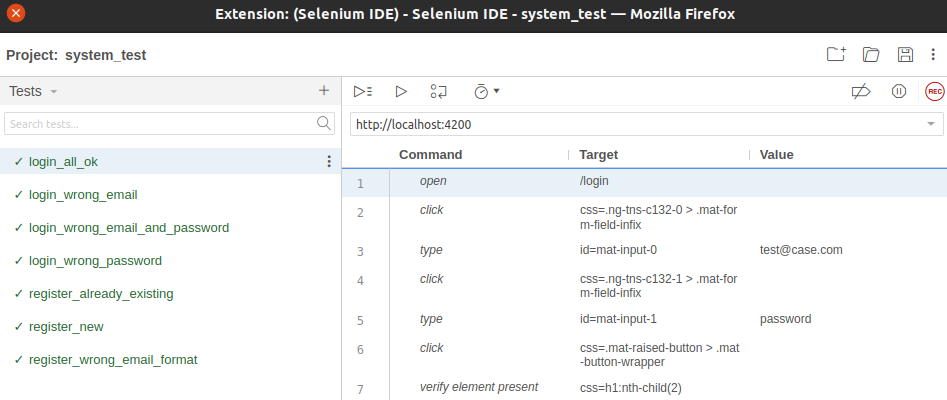
\includegraphics[width=\textwidth]{slike/tests_system/login_all_ok.png} %veličina u odnosu na širinu linije
                \caption{Testiranje uspješne prijave na stranicu}
                \label{fig:struktura} %label mora biti drugaciji za svaku sliku
            \end{figure}
            Prikazani su koraci testiranja gdje se testira logiranje u aplikaciju ukoliko je sve ispravno naravljeno. Korišteni e-mail je "test@case.com" te lozinka "password". Očekivani rezultat je preusmjeravanje na home page, što se prepoznaje i verificira putem elemenata stranice. Sa slike je vidljivo da se postiže očekivai rezultat.

            \begin{figure}[H]
                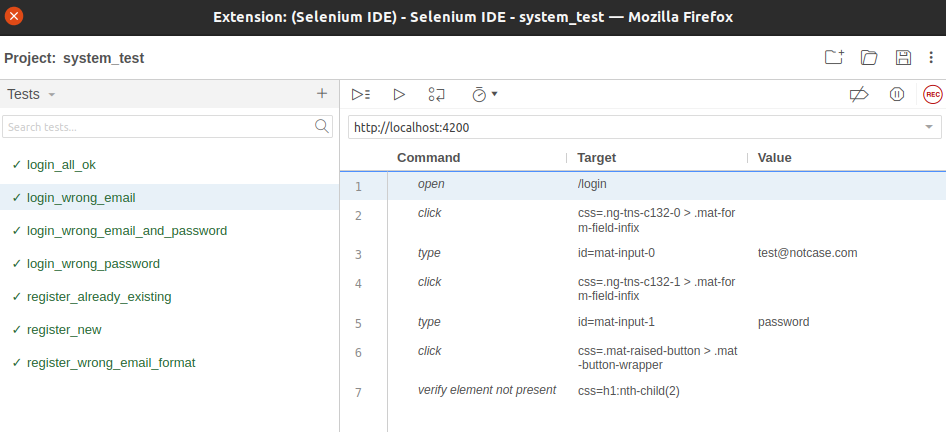
\includegraphics[width=\textwidth]{slike/tests_system/login_wrong_email.png} %veličina u odnosu na širinu linije
                \caption{Testiranje prijave neispravnim e-mailom}
                \label{fig:struktura} %label mora biti drugaciji za svaku sliku
            \end{figure}
            Prikazani su koraci testiranja gdje se testira logiranje u aplikaciju ukoliko je kriv e-mail. Korišteni e-mail je "test@notcase.com" te lozinka "password". Očekivani rezultat je ostajanje na login stranici, što se prepoznaje i verificira putem elemenata stranice. Sa slike je vidljivo da se postiže očekivai rezultat.

            \begin{figure}[H]
                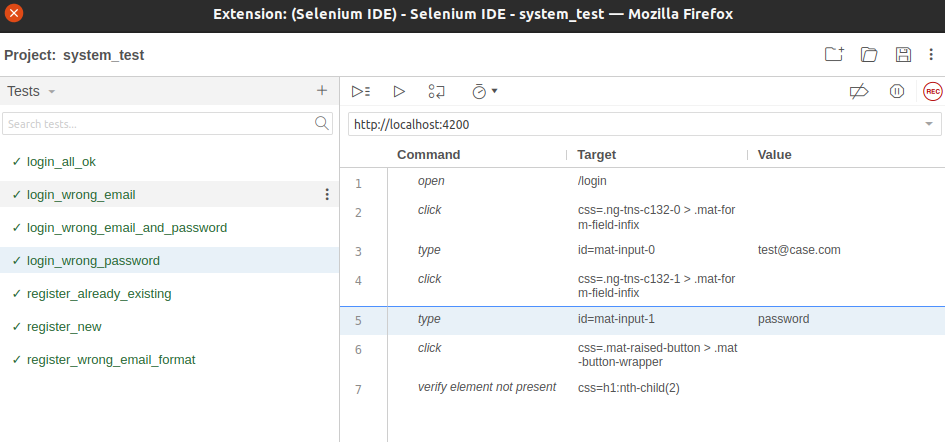
\includegraphics[width=\textwidth]{slike/tests_system/login_wrong_password.png} %veličina u odnosu na širinu linije
                \caption{Testiranje prijave neispravnom lozinkom}
                \label{fig:struktura} %label mora biti drugaciji za svaku sliku
            \end{figure}
            Prikazani su koraci testiranja gdje se testira logiranje u aplikaciju ukoliko je kriva lozinka. Korišteni e-mail je "test@case.com" te lozinka "password2". Očekivani rezultat je ostajanje na login stranici, što se prepoznaje i verificira putem elemenata stranice. Sa slike je vidljivo da se postiže očekivai rezultat.

            \begin{figure}[H]
                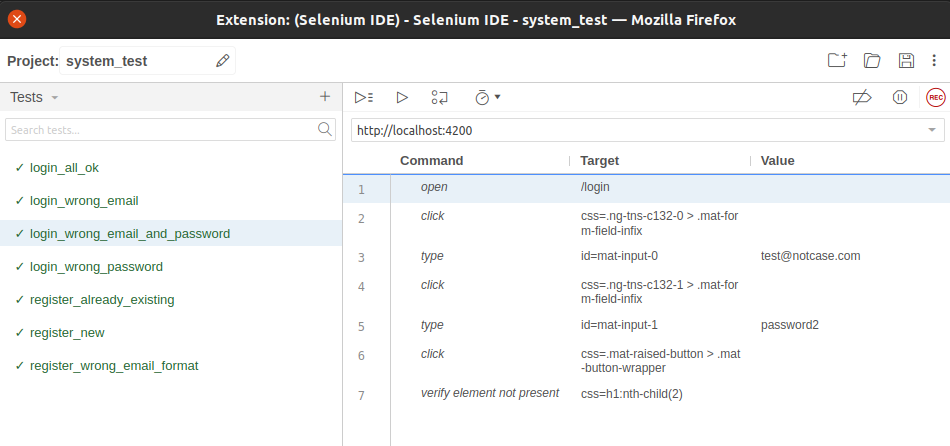
\includegraphics[width=\textwidth]{slike/tests_system/login_wrong_email_and_password.png} %veličina u odnosu na širinu linije
                \caption{Testiranje prijave neispravnom lozinkom i neispravnim e-mailom}
                \label{fig:struktura} %label mora biti drugaciji za svaku sliku
            \end{figure}
            Prikazani su koraci testiranja gdje se testira logiranje u aplikaciju ukoliko je kriva lozinka i e-mail. Korišteni e-mail je "test@notcase.com" te lozinka "password2". Očekivani rezultat je ostajanje na login stranici, što se prepoznaje i verificira putem elemenata stranice. Sa slike je vidljivo da se postiže očekivai rezultat.

            \begin{figure}[H]
                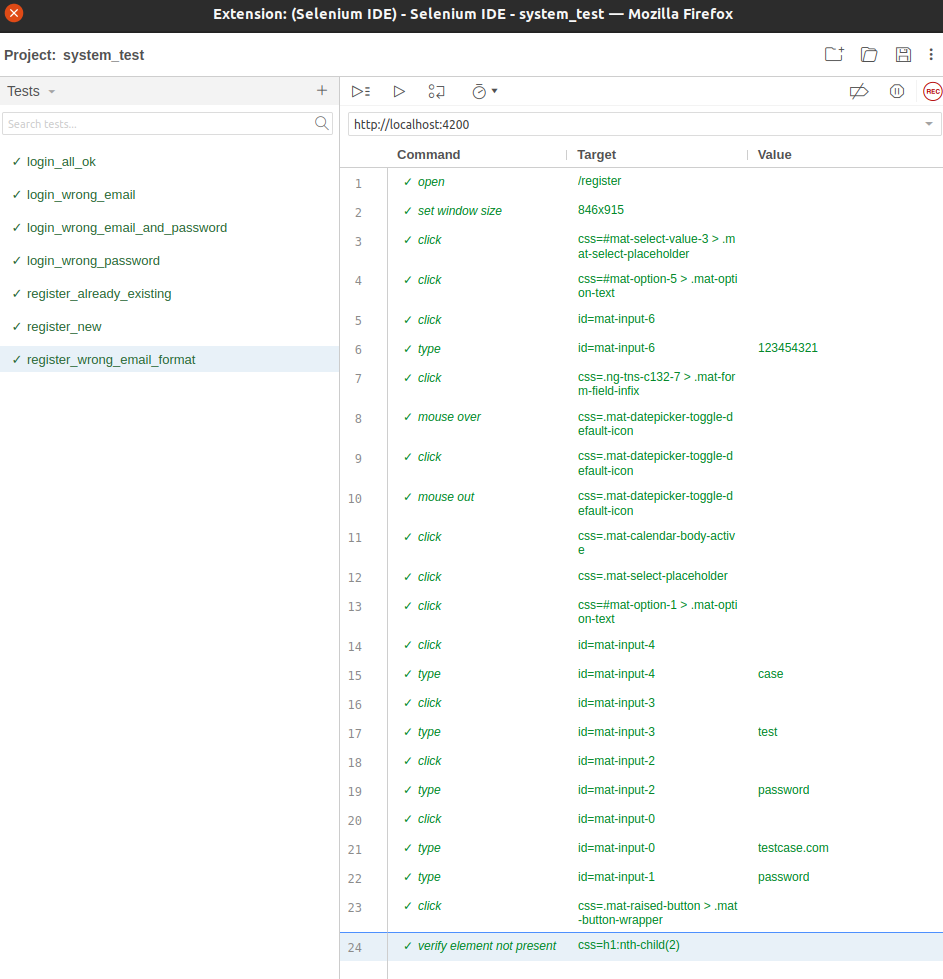
\includegraphics[width=\textwidth]{slike/tests_system/register_wrong_format.png} %veličina u odnosu na širinu linije
                \caption{Testiranje neuspješne registracije neispravnim e-mailom}
                \label{fig:struktura} %label mora biti drugaciji za svaku sliku
            \end{figure}
            Prikazani su koraci testiranja gdje se testira registracija korisnika gdje je sve ispravno napravljeno. Korišteni e-mail je "testcase.com", lozinka i ponovljena lozinka "password", ime "test", prezime "case", broj mobitela "123456789" te datum rođenja izabran putem date selectora. Očekivani rezultat je ostajanje na register stranici, što se prepoznaje i verificira putem elemenata stranice. Sa slike je vidljivo da se postiže očekivani rezultat.

            \begin{figure}[H]
                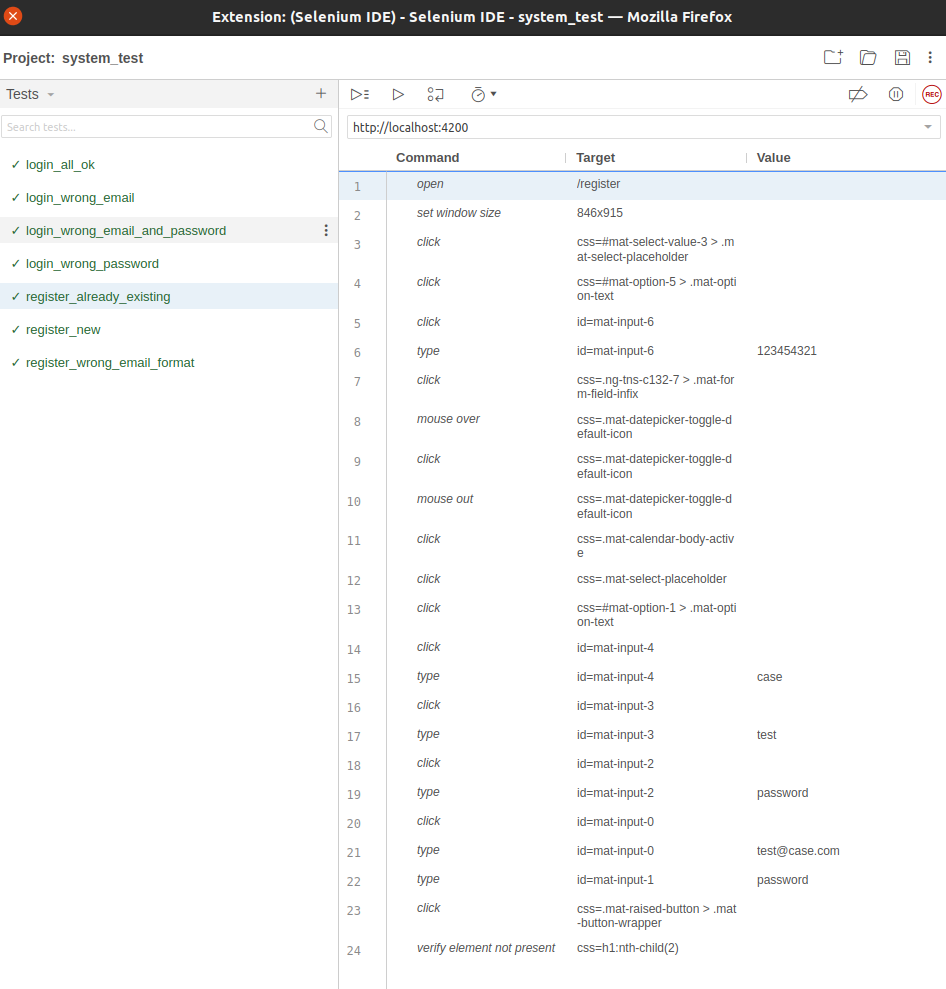
\includegraphics[width=\textwidth]{slike/tests_system/register_already_existing.png} %veličina u odnosu na širinu linije
                \caption{Testiranje neuspješne registracije već korištenim e-mailom}
                \label{fig:struktura} %label mora biti drugaciji za svaku sliku
            \end{figure}
            Prikazani su koraci testiranja gdje se testira registracija korisnika gdje je sve ispravno napravljeno. Korišteni e-mail je "test@case.com", lozinka i ponovljena lozinka "password", ime "test", prezime "case", broj mobitela "123456789" te datum rođenja izabran putem date selectora. User s prikazanim e-mailom je već registriran. Očekivani rezultat je ostajanje na register stranici, što se prepoznaje i verificira putem elemenata stranice. Sa slike je vidljivo da se postiže očekivai rezultat.

            \begin{figure}[H]
                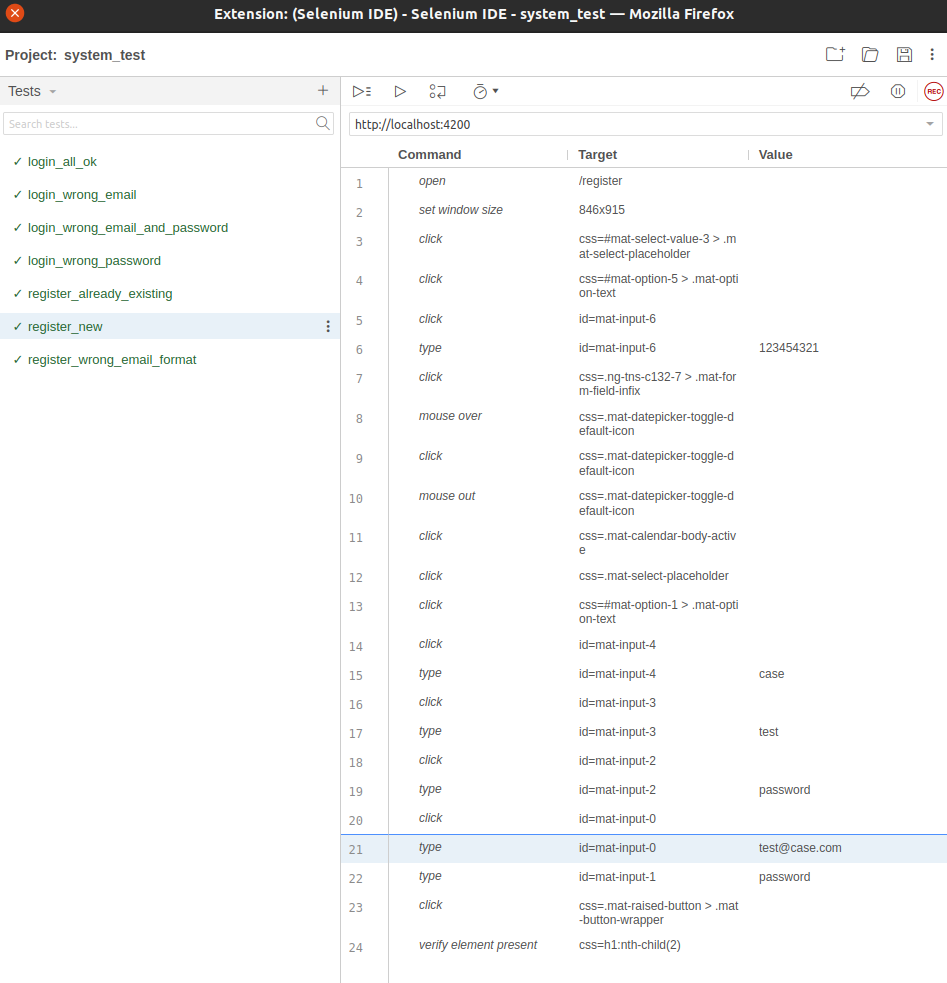
\includegraphics[width=\textwidth]{slike/tests_system/register_new.png} %veličina u odnosu na širinu linije
                \caption{Testiranje uspješne registracije}
                \label{fig:struktura} %label mora biti drugaciji za svaku sliku
            \end{figure}
            Prikazani su koraci testiranja gdje se testira registracija korisnika gdje je sve ispravno napravljeno. Korišteni e-mail je "test@case.com", lozinka i ponovljena lozinka "password", ime "test", prezime "case", broj mobitela "123456789" te datum rođenja izabran putem date selectora. Očekivani rezultat je preusmjeravanje na home stranicu, što se prepoznaje i verificira putem elemenata stranice. Sa slike je vidljivo da se postiže očekivani rezultat.
            
            \eject
		
		\section{Dijagram razmještaja}
			
			%\textbf{\textit{dio 2. revizije}}
			
			 %\textit{Potrebno je umetnuti %\textbf{specifikacijski} dijagram razmještaja i opisati ga. Moguće je umjesto specifikacijskog dijagrama razmještaja umetnuti dijagram razmještaja instanci, pod uvjetom da taj dijagram bolje opisuje neki važniji dio sustava.}
			 
			 Na slici 5.12 prikazan je dijagram razmještaja. Sustav je baziran na arhitekturi ”klijent-poslužitelj”. Korisnici pristupaju aplikaciji korištenjem web preglednika. Na platformi Microsoft Azure u VM-u (virtualnom stroju) se nalaze poslužitelji za frontend, backend i bazu podataka. Komunikacija između korisnika i poslužitelja za frontend, poslužitelja za frontend i poslužitelja za backend, ostvaruje se korištenjem protokola HTTP.
			 
			 
			 
			 \begin{figure}[H]
			            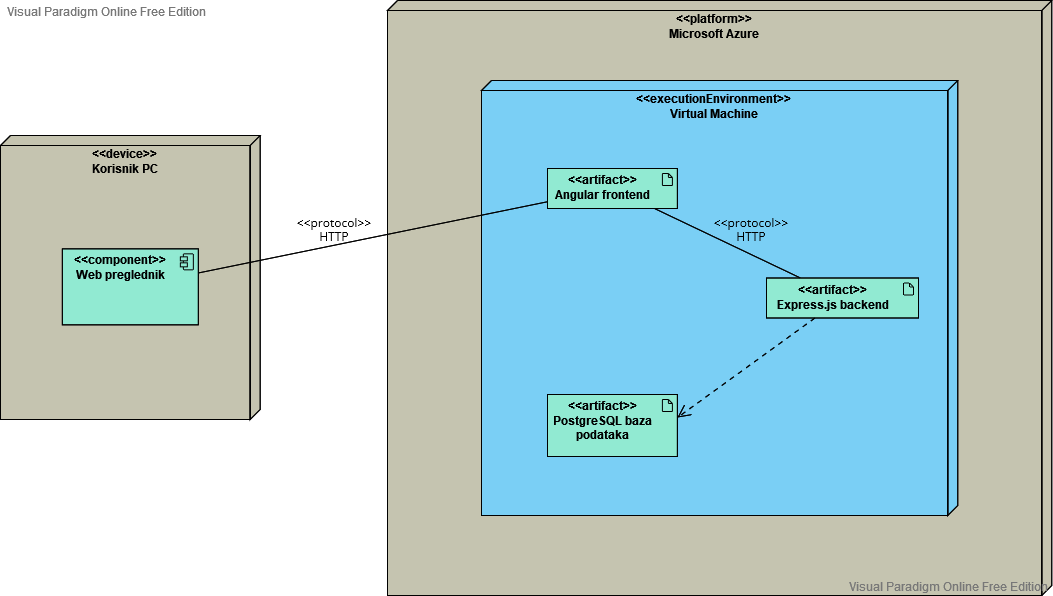
\includegraphics[width=\textwidth]{slike/Dijagram_razmjestaja_v2.png} %veličina u odnosu na širinu linije
			          \caption{Dijagram razmještanja}
			            \label{fig:dijagram_razmjestanja} %label mora biti drugaciji za svaku sliku
		      \end{figure}
			
			\eject 
		
		\section{Upute za puštanje u pogon}
				
			 Puštanje u pogon sastoji se od nekoliko koraka:
    \begin{itemize}
		\item 	\textit{Izrada koričkog računa na Microsoftovom Azure servisu}
		\item 	\textit{Zauzimanje nove virtualne mašine}
		\item 	\textit{Logiranje u novu virtualnu mašinu}
		\item 	\textit{Instaliranje potrebnih knjižnica i programa te downloadanje programa}
		\item 	\textit{Punjenje Postgres baze podataka}
		\item 	\textit{Pokretanje aplikacije s pripadajućom skriptom}
	\end{itemize}

    \subsection{Izrada koričkog računa na Microsoftovom Azure servisu}
    Potrebno je posjetiti stranicu azure.com te napraviti korisnichki račun.

    \subsection{Zauzimanje nove virtualne mašine}
    Potrebno je na svojem home pageu na Azureovom servisu zauzeti novu virtualnu mašinu. Za to je potrebno pritisnuti na "Virtual Machine" te pratiti potrebne korake koji automatski dolaze jedan iza drugoga. Također je potrebno dopustiti konekciju na port 80.
    \begin{figure}[H]
        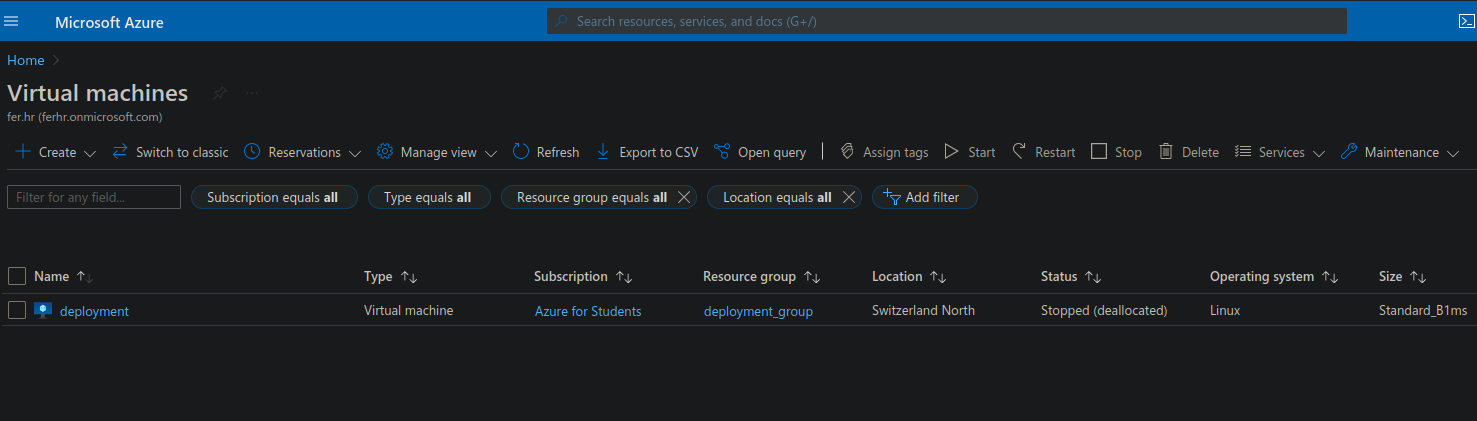
\includegraphics[width=\textwidth]{slike/deploy/create_vm.png} %veličina u odnosu na širinu linije
        \caption{Prikaz stanja stranice kada se odabere kreiranje virtualne mašine.}
        \label{fig:struktura} %label mora biti drugaciji za svaku sliku
    \end{figure}

    \subsection{Logiranje u novu virtualnu mašinu}
    Na home pageu potrebno je odabrati virtualnu mašinu te stisnuti na "Start" te zatim "Connect" i izabrati ssh. Zatim pratiti upute koje Azure navodi.
    \begin{figure}[H]
        
\includegraphics[width=\textwidth]{slike/deploy/connect.png} %veličina u odnosu na širinu linije
        \caption{Logiranje u novu virtualnu mašinu}
        \label{fig:struktura} %label mora biti drugaciji za svaku sliku
    \end{figure}
    Prikaz opcija koje su vidljive na vrhu ekrana nakon što je odabrana virtualna mašina. Potrebno je stisnuti "Start", a zatim i "Connect", odabrati SSH i pratiti upute.

    \subsection{Instaliranje potrebnih knjižnica i programa te downloadanje programa}
    Potrebno je klonirati program backenda i frontenda na virtualnu mašin pomoću komande "git clone <insert-url>", sustav će pitati za korisnika i lozinku. Nadalje trebamo instalirati sve potrebno za rad kloniranoga repozitorija. To postižemo s "sudo apt install nodejs" za nodejs, "npm install -g @angular/cli" za angular, "sudo apt install postgresql postgresql-contrib" za Postgres. Također da smo sigurni da je Postgres upaljen treba provesti još "sudo systemctl start postgresql.service". Ostali dijelovi se dobivaju preko "npm install" u frontend i backend direktorijima.

    \subsection{Punjenje Postgres baze podataka}
    Potrebno je dodati u bazu podataka tablice koje se dalje koriste u backendu. Pozicionirati se u direktorij backenda ("cd sustav-narucivanja/sustav-narucivanja-server") te zatim "node db/seed.js"
    \begin{figure}[H]
        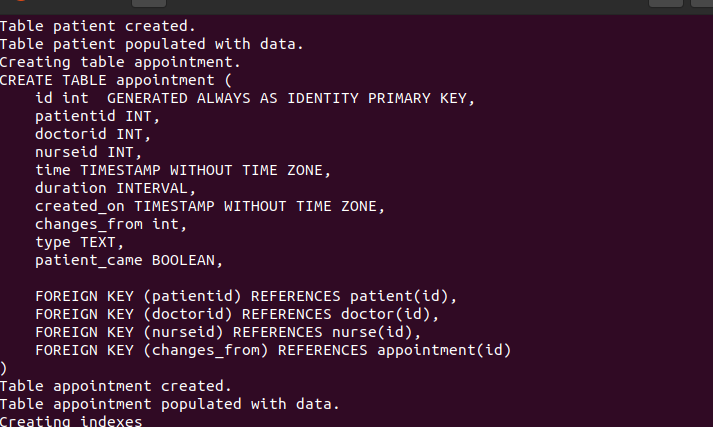
\includegraphics[width=\textwidth]{slike/deploy/seed.png} %veličina u odnosu na širinu linije
        \caption{Očekivani ispis prilikom pokretanja "seed.js".}
        \label{fig:struktura} %label mora biti drugaciji za svaku sliku
    \end{figure}
     Imati na umu da je ovo samo krajnji dio ispisa, postoji i dio prije ovoga koji je izbačen iz slike u svrhu sažetosti.

    \subsection{Pokretanje aplikacije}
    Potrebno je pokreniti restart skriptu koja se nalazi u root dijelu. Za to joj je potrebno dati ovlasti za pokretanje i onda je pokrenuti "sudo ./restart.sh"
			

			
			\eject 